\documentclass[aspectratio=169]{beamer}
\usepackage[utf8]{inputenc}
\usepackage[T1]{fontenc}
\usepackage{lmodern}
\usepackage{graphicx}
\usepackage{booktabs}
\usepackage{array}
\usepackage{listings}
\usepackage{tikz}
\usepackage{multicol}
\usepackage{ragged2e}
\usepackage{fontawesome5}
\usepackage{xcolor}
\usepackage{textpos}
\usepackage{appendixnumberbeamer}
\usetheme{Madrid}
\usecolortheme{seahorse}

% Custom colors
\definecolor{LPTABlue}{HTML}{2563EB}
\definecolor{LPTAGreen}{HTML}{10B981}
\definecolor{LPTARed}{HTML}{EF4444}
\definecolor{LPTAYellow}{HTML}{F59E0B}
\definecolor{codebg}{HTML}{0F172A}
\definecolor{codefg}{HTML}{DBE7FF}

\setbeamercolor{structure}{fg=LPTABlue}
\setbeamercolor{title}{fg=LPTABlue}
\setbeamercolor{frametitle}{fg=LPTABlue}
\setbeamercolor{normal text}{fg=black}
\setbeamercolor{alerted text}{fg=LPTARed}
\setbeamercolor{example text}{fg=LPTAGreen}

\setbeamertemplate{navigation symbols}{}
\setbeamertemplate{footline}[frame number]
\setbeamertemplate{caption}[numbered]

% Listings style
\lstdefinestyle{llvm}{
  basicstyle=\ttfamily\footnotesize\color{codefg},
  backgroundcolor=\color{codebg},
  frame=single,
  framesep=3pt,
  rulecolor=\color{LPTABlue!50},
  breaklines=true,
  columns=fullflexible,
  keepspaces=true,
  showstringspaces=false,
  language=LLVM,
}

\lstdefinestyle{bash}{
  basicstyle=\ttfamily\footnotesize\color{codefg},
  backgroundcolor=\color{codebg},
  frame=single,
  framesep=3pt,
  rulecolor=\color{LPTABlue!50},
  breaklines=true,
  columns=fullflexible,
  keepspaces=true,
  showstringspaces=false,
  language=bash,
}

\newcommand{\metric}[2]{\textbf{#1}: \texttt{#2}}
\newcommand{\red}[1]{\textcolor{LPTARed}{#1}}
\newcommand{\green}[1]{\textcolor{LPTAGreen}{#1}}
\newcommand{\blue}[1]{\textcolor{LPTABlue}{#1}}

\title{LPTA — LLVM Pass Transformation Analysis}
\subtitle{Making the Optimization Pipeline Transparent}
\author{Ramri}
\date{Segfault Hackathon 2025}
\institute{}

\begin{document}

% ============================================================
% SLIDE 1 — TITLE
% ============================================================
\begin{frame}
  \vfill
  \centering
  \begin{beamercolorbox}[sep=8pt,center]{title}
    \usebeamerfont{title}\LARGE LPTA\\[0.4em]
    \usebeamerfont{subtitle}\large LLVM Pass Transformation Analysis
  \end{beamercolorbox}
  \vspace{1.5em}
  \begin{beamercolorbox}[sep=4pt,center]{author}
    \usebeamerfont{author} Ramri
  \end{beamercolorbox}
  \begin{beamercolorbox}[sep=4pt,center]{date}
    \usebeamerfont{date} Segfault Hackathon 2025
  \end{beamercolorbox}
  \vspace{1em}
  \begin{beamercolorbox}[sep=4pt,center]{institute}
    \usebeamerfont{institute} \faGithub\ \texttt{github.com/rithesh-4/LPTA}
  \end{beamercolorbox}
  \vfill
\end{frame}

% ============================================================
% SLIDE 2 — THE PROBLEM
% ============================================================
\begin{frame}{The Problem: What Happens Inside \texttt{-O2}?}
  \begin{columns}[T,onlytextwidth]
    \begin{column}{0.55\textwidth}
      \begin{block}{The Black Box}
        \texttt{clang -O2} runs \textbf{878 pass executions} on your IR.\\
        You see input. You see output.\\
        \textbf{You have no idea what happened in between.}
      \end{block}
      \begin{alertblock}{Native LLVM Tools}
        \begin{itemize}
          \item \texttt{-print-before-all} / \texttt{-print-after-all} $\to$ 2,000+ lines of raw IR
          \item \texttt{-debug-pass-manager} $\to$ pass names only, no metrics
          \item \texttt{opt -stats} $\to$ global counters, no per-pass breakdown
        \end{itemize}
        \textbf{None correlate: which pass changed what, and how significant?}
      \end{alertblock}
    \end{column}
    \begin{column}{0.4\textwidth}
      \centering
      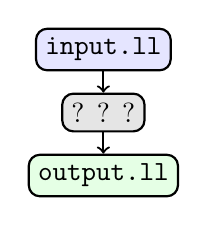
\begin{tikzpicture}[node distance=0.8cm]
        \node[draw,rounded corners,fill=blue!10,thick] (input) {\texttt{input.ll}};
        \node[draw,rounded corners,fill=gray!20,thick,below of=input] (box) {? ? ?};
        \node[draw,rounded corners,fill=green!10,thick,below of=box] (output) {\texttt{output.ll}};
        \draw[->,thick] (input) -- (box);
        \draw[->,thick] (box) -- (output);
      \end{tikzpicture}
      \vspace{1em}
      \small 878 pass executions $\times$ 2 events = \textbf{1,756 events} nobody can see
    \end{column}
  \end{columns}
\end{frame}

% ============================================================
% SLIDE 3 — VILLAIN SLIDE
% ============================================================
\begin{frame}[fragile]{The Villain: \texttt{opt -print-before-all}}
  \footnotesize
  \begin{lstlisting}[style=llvm]
; BEFORE: InstCombinePass
define i32 @foo(i32 %a) {
entry:
  %0 = add i32 %a, 1
  %1 = mul i32 %0, 2
  %2 = sub i32 %1, 3
  ret i32 %2
}
; AFTER: InstCombinePass
define i32 @foo(i32 %a) {
entry:
  %0 = add i32 %a, 1
  %1 = mul i32 %0, 2
  %2 = sub i32 %1, 3
  ret i32 %2
}
  \end{lstlisting}
  \vspace{-0.5em}
  \begin{alertblock}{}
    \textbf{2,000+ lines} of raw IR dumps. No metrics. No deltas. No correlation.\\
    \textbf{Zero insight.} Just noise.
  \end{alertblock}
  \vspace{-0.5em}
  \begin{columns}[T,onlytextwidth]
    \begin{column}{0.5\textwidth}
      \metric{Pass executions}{878}
    \end{column}
    \begin{column}{0.5\textwidth}
      \metric{Events recorded}{1,756}
    \end{column}
  \end{columns}
\end{frame}

% ============================================================
% SLIDE 4 — THE GOAL
% ============================================================
\begin{frame}{Goal: A Unified, Explainable View}
  \begin{block}{Problem Statement}
    \textit{``Developers lack a unified view that correlates which pass changed the IR,
    what changed, and how significant that change was.''}
  \end{block}
  \vspace{0.5em}
  \begin{columns}[T,onlytextwidth]
    \begin{column}{0.5\textwidth}
      \begin{itemize}
        \item Which passes ran?
        \item What did each one change?
        \item How significant was each change?
        \item How did it affect final codegen?
      \end{itemize}
    \end{column}
    \begin{column}{0.5\textwidth}
      \begin{alertblock}{Expected Outcome}
        An \textbf{explainable, evidence-backed view} of LLVM's
        optimization pipeline — turning manual, multi-stage IR
        comparison into a \textbf{repeatable workflow} for understanding
        optimization behavior and investigating regressions.
      \end{alertblock}
    \end{column}
  \end{columns}
\end{frame}

% ============================================================
% SLIDE 5 — WHAT LPTA DOES (ARCHITECTURE)
% ============================================================
\begin{frame}{What LPTA Does: End-to-End Pipeline}
  \centering
  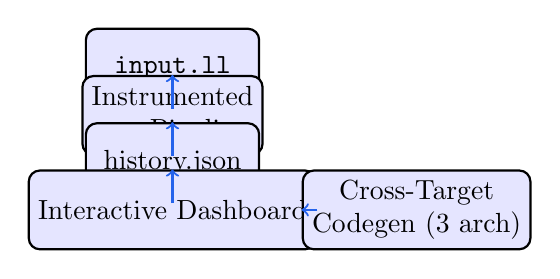
\begin{tikzpicture}[
    node distance=0.6cm and 1.2cm,
    box/.style={draw,rounded corners,fill=blue!10,thick,minimum width=2.2cm,minimum height=1cm,align=center},
    arrow/.style={->,thick,LPTABlue}
  ]
    \node[box] (input) {\texttt{input.ll}};
    \node[box,below of=input] (opt) {Instrumented\\ \texttt{opt} Pipeline};
    \node[box,below of=opt] (json) {history.json};
    \node[box,below of=json] (dash) {Interactive Dashboard};
    \node[box,right of=dash,xshift=2.5cm] (codegen) {Cross-Target\\ Codegen (3 arch)};
    \draw[arrow] (input) -- (opt);
    \draw[arrow] (opt) -- (json);
    \draw[arrow] (json) -- (dash);
    \draw[arrow] (dash) -- (codegen);
  \end{tikzpicture}
  \vspace{0.5em}
  \begin{multicols}{2}
    \begin{itemize}
      \item Instruments \textbf{every pass} via \texttt{PassInstrumentationCallbacks}
      \item Records IR state \textbf{before/after} each pass
      \item Computes \textbf{10 structural metrics} + deltas
      \item Saves IR snapshots for changed passes
      \item Measures codegen via \texttt{llc} (x86, aarch64, riscv64)
      \item Emits \texttt{history.json} + interactive HTML dashboard
    \end{itemize}
  \end{multicols}
\end{frame}

% ============================================================
% SLIDE 6 — ONE PASS END-TO-END (REAL DATA)
% ============================================================
\begin{frame}[fragile]{One Pass, End-to-End: SimplifyCFG on \texttt{demo\_input.ll}}
  \begin{columns}[T,onlytextwidth]
    \begin{column}{0.48\textwidth}
      \textbf{Before (17 instr, 4 BB, 3 branches, 1 phi)}
      \begin{lstlisting}[style=llvm]
define i32 @foo(i32 %a) {
entry:
  %cmp = icmp sgt i32 %a, 100
  br i1 %cmp, label %big, label %small
big:
  %x1 = add i32 %a, 1
  %x2 = mul i32 %x1, 2
  ...
  br label %merge
small:
  br label %merge
merge:
  %phi = phi i32 [%x6, %big], [42, %small]
  ret i32 %phi
}
      \end{lstlisting}
    \end{column}
    \begin{column}{0.48\textwidth}
      \textbf{After (14 instr, 1 BB, 0 branches, 0 phi)}
      \begin{lstlisting}[style=llvm]
define i32 @foo(i32 %a) {
entry:
  %cmp = icmp sgt i32 %a, 100
  %spec = select i1 %cmp, i32 999, i32 42
  ret i32 %spec
}
      \end{lstlisting}
      \vspace{0.5em}
      \begin{tabular}{lrrr}
        \toprule
        Metric & Before & After & \textbf{Delta} \\
        \midrule
        Instructions & 17 & 14 & \red{-3} \\
        Basic Blocks & 4 & 1 & \red{-3} \\
        Branches & 3 & 0 & \red{-3} \\
        PHIs & 1 & 0 & \red{-1} \\
        \bottomrule
      \end{tabular}
      \vspace{0.5em}
      \green{\textbf{Stack remaining: 0}} — pass nesting balanced
    \end{column}
  \end{columns}
\end{frame}

% ============================================================
% SLIDE 7 — DASHBOARD (PLACEHOLDER)
% ============================================================
\begin{frame}{Dashboard: The Explainable View}
  \centering
  \vspace{1em}
  \fbox{\begin{minipage}{0.85\textwidth}
    \centering
    \vspace{2em}
    \large \texttt{[ DASHBOARD SCREENSHOT ]}\\
    \vspace{0.5em}
    \small Overview | Pipeline Timeline | Functions | Pass Explorer (IR Diff) | Compare
    \vspace{2em}
  \end{minipage}}
  \vspace{0.5em}
  \small \textit{Placeholder — insert screenshot from \texttt{http://localhost:8080/} Overview page}
  \vspace{1em}
  \begin{alertblock}{Key Features}
    \begin{itemize}
      \item Summary cards: 1,756 events, 102 changed passes, 109$\to$112 instr, 190$\to$219 asm
      \item Pipeline timeline: 878 executions visualized (red = changed)
      \item Pass Explorer: filterable, click any pass $\to$ IR diff modal
      \item Compare tab: load two \texttt{history.json} $\to$ regression score + findings
    \end{itemize}
  \end{alertblock}
\end{frame}

% ============================================================
% SLIDE 8 — AGGREGATION TABLE
% ============================================================
\begin{frame}{What Changed + How Significant: Aggregated Impact}
  \begin{tabular}{lrrrrr}
    \toprule
    Pass & \# Executions & Instr $\Delta$ & BB $\Delta$ & Branches $\Delta$ & PHIs $\Delta$ \\
    \midrule
    SimplifyCFGPass       & 14 & \red{-42} & \red{-22} & \red{-31} & \red{-11} \\
    EarlyCSEPass          & 5  & \red{-19} & 0 & 0 & 0 \\
    InstCombinePass       & 6  & \red{-18} & 0 & 0 & 0 \\
    SROAPass              & 1  & \red{-10} & \red{-2} & 0 & 0 \\
    InstSimplifyPass      & 2  & \red{-7}  & 0 & 0 & 0 \\
    \midrule
    LoopVectorizePass     & 2  & \blue{+58}  & \blue{+10} & \blue{+12} & \blue{+15} \\
    FunctionToLoopPassAdaptor & 10 & \blue{+30} & \blue{+8} & \blue{+8} & \blue{+8} \\
    PassManager<Function> & 25 & \blue{+26} & \blue{+5} & \blue{+4} & \blue{+5} \\
    LoopUnrollPass        & 2  & \blue{+14} & \blue{+3} & \blue{+4} & \blue{+5} \\
    \bottomrule
  \end{tabular}
  \vspace{0.5em}
  \begin{block}{The Tradeoff}
    Cleanup passes remove 96 instructions; vectorization/unrolling adds 102.\\
    Net: \red{+3 instr}, but \green{BBs -21\%}, \blue{codegen +15\%} (190 $\to$ 219 asm lines).
  \end{block}
\end{frame}

% ============================================================
% SLIDE 9 — CROSS-TARGET CODEGEN
% ============================================================
\begin{frame}{Cross-Target Codegen: Same Pipeline, Three Architectures}
  \begin{tabular}{lrrrrrr}
    \toprule
    Target & Before (lines) & After (lines) & $\Delta$ & Before (bytes) & After (bytes) \\
    \midrule
    x86\_64-pc-windows-msvc & 195 & 232 & \blue{+37 (+19\%)} & 5,241 & 6,469 \\
    aarch64-unknown-linux-gnu & 155 & 203 & \blue{+48 (+31\%)} & 4,834 & 6,359 \\
    riscv64-unknown-linux-gnu & 221 & 267 & \blue{+46 (+21\%)} & 6,207 & 7,257 \\
    \midrule
    \textbf{Total} & \textbf{190} & \textbf{219} & \blue{\textbf{+29 (+15\%)}} & \textbf{16,282} & \textbf{20,085} \\
    \bottomrule
  \end{tabular}
  \vspace{0.5em}
  \begin{block}{Insight}
    The \textbf{same optimized IR} produces different code-size impacts per architecture.\\
    aarch64 sees the largest relative increase (+31\%) due to different instruction-set cost
    modeling for the operations this code uses. \textbf{You cannot get this from \texttt{opt} alone.}
  \end{block}
\end{frame}

% ============================================================
% SLIDE 10 — CROSS-RUN COMPARE
% ============================================================
\begin{frame}{Cross-Run Regression Detection}
  \centering
  \vspace{1em}
  \fbox{\begin{minipage}{0.85\textwidth}
    \centering
    \vspace{1.5em}
    \large \texttt{[ COMPARE GAUGE SCREENSHOT ]}\\
    \vspace{0.5em}
    \small Regression Score: 13/100 — Mostly improvements with minor variations
    \vspace{1.5em}
  \end{minipage}}
  \vspace{0.5em}
  \small \textit{Placeholder — insert screenshot from Compare tab}
  \vspace{1em}
  \begin{columns}[T,onlytextwidth]
    \begin{column}{0.5\textwidth}
      \begin{alertblock}{Findings (O0 $\to$ O2 on \texttt{tiny\_proof.ll})}
        \begin{itemize}
          \item \green{Instruction reduction: 41\% (12 $\to$ 7)}
          \item \green{Codegen reduction: 10\% (40 $\to$ 36 asm lines)}
          \item \blue{5 new passes appeared:} EarlyCSE, InstCombine, SimplifyCFG, PassManager, ModuleToFunctionPassAdaptor
        \end{itemize}
      \end{alertblock}
    </column>
    \begin{column}{0.5\textwidth}
      \begin{block}{CLI Mode}
        \begin{lstlisting}[style=bash]
build/lpta_test.exe --compare \
  baseline/history.json \
  current/history.json
        \end{lstlisting}
        Identical analysis, CI-friendly output.
      \end{block}
    </column>
  </columns>
\end{frame}

% ============================================================
% SLIDE 11 — HOW WE DID IT DURING THE HACKATHON
% ============================================================
\begin{frame}[fragile]{How We Did It During the Hackathon}
  \begin{columns}[T,onlytextwidth]
    \begin{column}{0.55\textwidth}
      \begin{alertblock}{No Parser, No LLVM Fork}
        \begin{itemize}
          \item Hooked LLVM's \texttt{PassInstrumentationCallbacks}
          \item Runs the \textbf{real \texttt{-O2} pipeline} (not a simulation)
          \item Only 6 opcodes counted individually: call/invoke/callbr, load, store, br, phi, ret
          \item Everything else $\to$ \texttt{instruction\_count}
        \end{itemize}
      \end{alertblock}
      \begin{block}{Hook Registration}
        \begin{lstlisting}[style=bash]
PIC.registerBeforeNonSkippedPassCallback(
  [&](StringRef PassID, Any IR) {
    // capture before-metrics, push frame
  });
PIC.registerAfterPassCallback(
  [&](StringRef PassID, Any IR, PreservedAnalyses &PA) {
    // pop frame, capture after-metrics, delta, record event
  });
        \end{lstlisting}
      \end{block}
    \end{column}
    \begin{column}{0.4\textwidth}
      \begin{block}{Why a Stack?}
        \begin{itemize}
          \item Module $\to$ Function $\to$ Loop nesting
          \item Single ``current pass'' overwritten by inner passes
          \item Stack of \texttt{PassFrame} matches BEFORE/AFTER by IR-unit pointer
        \end{itemize}
        \vspace{1em}
        \metric{Depth 0}{Module}
        \metric{Depth 1}{Function}
        \metric{Depth 2}{Loop}
      \end{block}
    \end{column}
  \end{columns}
\end{frame}

% ============================================================
% SLIDE 12 — THE HARD PROBLEM: PASSFRAME STACK
% ============================================================
\begin{frame}{The Hard Problem: Nesting + Frame Matching}
  \centering
  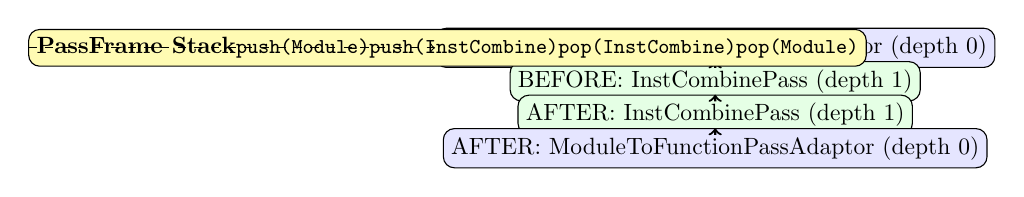
\begin{tikzpicture}[node distance=0.5cm, scale=0.85, transform shape]
    \node[draw,rounded corners,fill=blue!10] (m0) {BEFORE: ModuleToFunctionPassAdaptor (depth 0)};
    \node[draw,rounded corners,fill=green!10,below of=m0] (f0) {BEFORE: InstCombinePass (depth 1)};
    \node[draw,rounded corners,fill=green!10,below of=f0] (f1) {AFTER: InstCombinePass (depth 1)};
    \node[draw,rounded corners,fill=blue!10,below of=f1] (m1) {AFTER: ModuleToFunctionPassAdaptor (depth 0)};
    \draw[->,thick] (m0) -- (f0);
    \draw[->,thick] (f0) -- (f1);
    \draw[->,thick] (f1) -- (m1);
    \node[draw,rounded corners,fill=yellow!30,left of=m0,xshift=-3.5cm] (stack) {\textbf{PassFrame Stack}\\
    \ttfamily\small push(Module)\\
    \ttfamily\small push(InstCombine)\\
    \ttfamily\small pop(InstCombine)\\
    \ttfamily\small pop(Module)};
    \draw[->,dashed] (stack) -- (m0);
  \end{tikzpicture}
  \vspace{0.5em}
  \begin{block}{Match Strategy (Critical for Correctness)}
    \begin{enumerate}
      \item Primary: \textbf{IR-unit pointer identity} (\texttt{Module*}/\texttt{Function*}/\texttt{Loop*}) — stable between BEFORE/AFTER
      \item Fallback: pass name only (CGSCC passes, unsupported IR unit)
      \item Invariant: \textbf{Stack remaining = 0} (verified by \texttt{judge\_proof.sh})
    \end{enumerate}
  \end{block}
\end{frame}

% ============================================================
% SLIDE 13 — 7-LAYER VALIDATION
% ============================================================
\begin{frame}{How Do You Know the Numbers Are Right? — 7-Layer Validation}
  \begin{tabular}{ll}
    \toprule
    \# & Layer \\
    \midrule
    1 & Hand-countable ground truth (\texttt{tiny\_proof.ll}: 2 fn, 12 instr, 10/10 match) \\
    2 & Independent IR parsing (grep-based recount vs. C++ counters) \\
    3 & LLVM cross-validation (\texttt{opt -stats} within tolerance) \\
    4 & Determinism (same input $\to$ byte-identical \texttt{history.json}) \\
    5 & Formal invariants (\texttt{assert}: instr $\ge$ call+load+store, BB $\ge$ ret) \\
    6 & 57 unit tests (invoke/callbr, delta math, JSON escaping, pass classification) \\
    7 & 300-iteration fuzz (crash/hang/corrupt-output free) \\
    \bottomrule
  \end{tabular}
  \vspace{0.5em}
  \begin{alertblock}{Run It Yourself}
    \begin{lstlisting}[style=bash]
bash tests/judge_proof.sh build/          # 10/10 exact match
bash tests/validate_correctness.sh build/ test.ll  # grep + opt cross-check
bash tests/run_all_tests.sh build/        # full suite (incl. fuzz)
    \end{lstlisting}
  \end{alertblock}
\end{frame}

% ============================================================
% SLIDE 14 — UNIT TESTS + FUZZ + DETERMINISM
% ============================================================
\begin{frame}{Unit Tests + Fuzz + Determinism}
  \begin{columns}[T,onlytextwidth]
    \begin{column}{0.5\textwidth}
      \begin{block}{57 Unit Tests (\texttt{test\_utilities.exe})}
        \begin{itemize}
          \item IRMetrics: zero-init, delta math, unsigned overflow safety
          \item JSON escaping: quotes, backslash, control chars, UTF-8 passthrough
          \item classifyPass: adaptor/pipeline/transformation/analysis priority
          \item invoke/callbr counted as calls; module vs function agreement
          \item sanitizeFilename: special chars, empty, dots preserved
        \end{itemize}
        \green{57/57 passed}
      \end{block}
    \end{column}
    \begin{column}{0.5\textwidth}
      \begin{block}{300-Iteration Fuzz}
        \begin{itemize}
          \item Mutations: truncate, insert random bytes, delete chunks, bit flips, heap spray, empty, null byte
          \item 30-second timeout per run
          \item \green{0 crashes, 0 timeouts}
        \end{itemize}
      \end{block}
      \begin{block}{Determinism}
        \begin{itemize}
          \item Two runs $\to$ byte-identical \texttt{history.json}
          \item Verified by \texttt{judge\_proof.sh} and \texttt{validate\_correctness.sh}
        \end{itemize}
      \end{block}
    \end{column}
  \end{columns}
\end{frame}

% ============================================================
% SLIDE 15 — LIMITATIONS (HONESTY SLIDE)
% ============================================================
\begin{frame}{Limitations — What LPTA Does \textbf{Not} Do}
  \begin{alertblock}{Calibrated Claims}
    \begin{itemize}
      \item \textbf{Counts structure, not speed.} Fewer instructions $\neq$ faster runtime. Significance score is a heuristic.
      \item \textbf{No runtime profiling.} No PGO, no cache-miss modeling, no hardware counters.
      \item \textbf{Heuristic pass classification.} Name-based (Adaptor, PassManager, Analysis) — could misclassify unusual passes.
      \item \textbf{6 opcodes only.} call/invoke/callbr, load, store, br, phi, ret. All arithmetic/logic/cast folded into \texttt{instruction\_count}.
      \item \textbf{Snapshots allowlisted + 4 MiB cap.} Only 12 high-impact passes emit IR text; large functions drop snapshots.
      \item \textbf{Single-threaded.} LLVM's pass pipeline is single-threaded; LPTA's callbacks rely on this.
    \end{itemize}
  \end{alertblock}
  \vspace{0.5em}
  \begin{block}{What It \textbf{Does} Do Well}
    Structural IR deltas per pass, cross-target codegen comparison, cross-run regression detection, deterministic evidence-backed trace.
  \end{block}
\end{frame}

% ============================================================
% SLIDE 16 — ROADMAP + THANK YOU
% ============================================================
\begin{frame}{Roadmap + Thank You}
  \begin{columns}[T,onlytextwidth]
    \begin{column}{0.5\textwidth}
      \begin{block}{Next (Post-Hackathon)}
        \begin{itemize}
          \item CI gating: \texttt{lpta\_test --compare} in PR pipeline
          \item Per-function codegen diff in Compare tab
          \item Export to SARIF for static-analysis tooling
          \item Windows/macOS/Linux binary releases
          \item AI Insights: local model support (Ollama), offline summaries
        \end{itemize}
      \end{block}
    \end{column}
    \begin{column}{0.5\textwidth}
      \begin{block}{Links}
        \begin{itemize}
          \item \faGithub\ \texttt{github.com/rithesh-4/LPTA}
          \item \faFileCode\ \texttt{README.md} — full usage guide
          \item \faFlask\ \texttt{tests/} — 7-layer validation suite
          \item \faQuestionCircle\ Issues welcome
        \end{itemize}
      \end{block}
    \end{column}
  \end{columns}
  \vspace{1em}
  \centering
  \Large \textbf{Thank You}
  \vspace{0.5em}
  \normalsize \texttt{bash run\_lpta.sh your\_code.ll --snapshots --targets=common}
\end{frame}

\end{document}